\documentclass[电力电子]{subfiles}
\begin{document}
\section{选择题}
\begin{ti}
	晶闸管导通的条件是\kuo{A}。
	\twoch{阳极加正向电压,门极有正向脉冲}{阳极加正向电压,门极有负向脉冲}{阳极加反向电压,门极有正向脉冲}{阳极加反向电压,门极有负向脉冲}
\end{ti}

\begin{ti}
	单相半波可控整流电路,阻性负载,控制角 $\alpha$ 的最大移相范围是 $0^\circ \sim $ \kuo{D}。
	\fourch{$90^\circ$}{$120^\circ$}{$150^\circ$}{$180^\circ$}
\end{ti}

\begin{ti}
	单相桥式整流电路,电阻性负载,控制角 $\alpha$ 为\kuo{D}时,整流输出电压为 $0$。
	\fourch{$0^\circ$}{$90^\circ$}{$120^\circ$}{$180^\circ$}
\end{ti}

\begin{ti}
	大电感性负载的三相半波整流电路,流过晶闸管的平均电流为\kuo{B}。
	\fourch{$\frac{1}{2} I_{\dd}$}{$\frac{1}{3} I_{\dd}$}{$\frac{\sqrt{2}}{2} I_{\dd}$}{$\frac{\sqrt{3}}{3} I_{\dd}$}
\end{ti}

\begin{ti}
	PWM 斩波电路一般采用\kuo{A}。
	\fourch{定频调宽控制}{定宽调频控制}{调频调宽控制}{瞬时值控制}
\end{ti}

\begin{ti}
	电压型逆变器,交流侧电压波形为\kuo{B}。
	\fourch{正弦波}{矩形波}{锯齿波}{梯形波}
\end{ti}

\begin{ti}
	单相全波可控整流电路,电感性负载,控制角 $\alpha \leq 30^\circ$,每个周期内输出电压的平均值为\kuo{B}。
	\fourch{$U_{\dd} = 0.45 U_{2} \cos \alpha$}{$U_{\dd} = 0.9 U_{2} \cos \alpha$}{$U_{\dd} = 1.17 U_{2} \cos \alpha$}{$U_{\dd} = 2.34 U_{2} \cos \alpha$}
\end{ti}

\begin{ti}
	三相全控制桥式有源逆变电路,在交流电源一个周期里,输出电压脉动次数\kuo{D}。
	\fourch{2}{3}{4}{6}
\end{ti}

\begin{ti}
	直流斩波器是:\kuo{D}。
	\fourch{AC/DC变换器}{DC/AC变换器}{AC/AC变换器}{DC/DC变换器}
\end{ti}

\begin{ti}
	PWM 脉宽调制技术用于\kuo{B}。
	\fourch{有源逆变器}{无源逆变器}{脉冲触发器}{脉冲移相器}
\end{ti}

\begin{ti}
	下列器件中为全控型器件的是\kuo{D}。
	\fourch{双向晶闸管}{快速晶闸管}{光控晶闸管}{功率场效应晶体管}
\end{ti}

\begin{ti}
	单相半波可控整流电路,带电阻负载,控制角 $\alpha$ 的最大移相范围为\kuo{B}。
	\fourch{$0^\circ \sim 90^\circ$}{$0^\circ \sim 180^\circ$}{$0^\circ \sim 120^\circ$}{$0^\circ \sim 150^\circ$}
\end{ti}

\begin{ti}
	单相半控桥,带大电感负载,直流侧并联续流管的主要作用是\kuo{A}。
	\fourch{防止失控现象}{减小输出电压的脉动}{减小输出电流的脉动}{直流侧过电压保护}
\end{ti}

\begin{ti}
	三相全控桥式整流电路,控制角 $\alpha$ 为\kuo{A}时,整流输出电压为最大值。
	\fourch{$0^\circ$}{$90^\circ$}{$120^\circ$}{$180^\circ$}
\end{ti}

\begin{ti}
	单相半波整流电路中,晶闸管可能承受的反向峰值电压为\kuo{B}。
	\fourch{$U_{2}$}{$\sqrt{2} U_{2}$}{$\sqrt{3} U_{2}$}{$\sqrt{6} U_{2}$}
\end{ti}

\begin{ti}
	三相半波可控整流电路,电阻性负载,控制角 $\alpha \leq 30^\circ$,每个周期内输出电压的平均值为\kuo{C}。
	\fourch{$U_{\dd} = 0.45 U_{2} \cos \alpha$}{$U_{\dd} = 0.9 U_{2} \cos \alpha$}{$U_{\dd} = 1.17 U_{2} \cos \alpha$}{$U_{\dd} = 2.34 U_{2} \cos \alpha$}
\end{ti}

\begin{ti}
	三相全控桥式整流电路,晶闸管可能承受的最大反向电压为\kuo{C}。
	\fourch{$\sqrt{3} U_{2}$}{$2\sqrt{2} U_{2}$}{$\sqrt{6} U_{2}$}{$2\sqrt{3} U_{2}$}
\end{ti}

\begin{ti}
	三相桥式全控整流电路,在交流电源一个周期里,输出电压脉动\kuo{D}次。
	\fourch{2}{3}{4}{6}
\end{ti}

\begin{ti}
	三相半波可控整流电路中三个晶闸管的触发脉冲相位互差\kuo{C}。
	\fourch{$60^\circ$}{$90^\circ$}{$120^\circ$}{$180^\circ$}
\end{ti}

\begin{ti}
	串联谐振式逆变电路晶闸管的换流方式为\kuo{C}。
	\fourch{器件换流}{电网换流}{负载换流}{脉冲换流}
\end{ti}

\begin{ti}
	晶闸管在导通状态下,管耗等于管子两端电压乘以\kuo{A}。
	\twoch{阳极电流}{门极电流}{阳极电流与门极电流之和}{阳极电流与门极电流之差}
\end{ti}

\begin{ti}
	单相半波可控整流电路,阻性负载,导通角 $\theta$ 的最大变化范围是 $0^\circ \sim $ \kuo{D}。
	\fourch{$90^\circ$}{$120^\circ$}{$150^\circ$}{$180^\circ$}
\end{ti}

\begin{ti}
	三相半波可控整流电路,阻性负载,导通角 $\theta$ 的最大变化范围是 $0^\circ \sim $ \kuo{C}。
	\fourch{$90^\circ$}{$120^\circ$}{$150^\circ$}{$180^\circ$}
\end{ti}

\begin{ti}
	三相全控桥式整流电路,阻性负载,导通角 $\theta$ 的最大变化范围是 $0^\circ \sim $ \kuo{B}。
	\fourch{$90^\circ$}{$120^\circ$}{$150^\circ$}{$180^\circ$}
\end{ti}

\begin{ti}
	三相半波可控整流电路电源电压波形的自然换向点比单相半波可控整流电路的自然换向点\kuo{B}。
	\fourch{超前 $30^\circ$}{滞后 $30^\circ$}{超前 $60^\circ$}{滞后 $60^\circ$}
\end{ti}

\begin{ti}
	单相全波可控整流电路,电感性负载,控制角 $\alpha \leq 30^\circ$,每个周期内输出电压的平均值为\kuo{B}。
	\fourch{$U_{\dd} = 0.45 U_{2} \cos \alpha$}{$U_{\dd} = 0.9 U_{2} \cos \alpha$}{$U_{\dd} = 1.17 U_{2} \cos \alpha$}{$U_{\dd} = 2.34 U_{2} \cos \alpha$}
\end{ti}

\begin{ti}
	三相全控桥式整流电路,电感性负载,控制角 $\alpha > 30^\circ$,负载电流连续,整流输出电流的平均值为 $I_{\dd}$,流过每只晶闸管的平均值电流为\kuo{B}。
	\fourch{$\frac{I_{\dd}}{2}$}{$\frac{I_{\dd}}{3}$}{$\frac{2I_{\dd}}{3}$}{$I_{\dd}$}
\end{ti}

\begin{ti}
	单相全控桥式有源逆变电路最小逆变角 $\beta$ 为\kuo{D}。
	\fourch{$1^\circ \sim 3^\circ$}{$10^\circ \sim 15^\circ$}{$20^\circ \sim 25^\circ$}{$30^\circ \sim 35^\circ$}
\end{ti}

\begin{ti}
	三相全控制桥式有源逆变电路,在交流电源一个周期里,输出电压脉动\kuo{D}次。
	\fourch{2}{3}{4}{6}
\end{ti}

\begin{ti}
	有源逆变电路是\kuo{B}。
	\fourch{AC/DC 变换器}{DC/AC 变换器}{AC/AC 变换器}{DC/DC 变换器}
\end{ti}

\begin{ti}
	晶闸管门极触发信号刚从断态转入通态即移去触发信号,能维持通态所需要的最小阳极电流,称为\kuo{B}。
	\fourch{维持电流}{擎住电流}{浪涌电流}{额定电流}
\end{ti}

\begin{ti}
	晶闸管门极触发信号刚从断态转入通态即移去触发信号,能维持通态所需要的最小阳极电流,称为\kuo{B}。
	\fourch{维持电流}{擎住电流}{浪涌电流}{额定电流}
\end{ti}

\begin{ti}
	为了减小门极损耗,晶闸管正常导通的方法是阳极加正向电压,门极加\kuo{A}。
	\fourch{正脉冲}{负脉冲}{直流}{正弦波}
\end{ti}

\begin{ti}
	在 GTR 作为开关的电路中,若在转换的过程中出现从高电压小电流到低电压大电流的现象,则说明晶体管\kuo{B}。
	\fourch{失控}{二次击穿}{不能控制关断}{不能控制开通}
\end{ti}

\begin{ti}
	下列器件中为全控型器件的是\kuo{D}。
	\fourch{双向晶闸管}{快速晶闸管}{光控晶闸管}{功率场效应晶体管}
\end{ti}

\begin{ti}
	单相半波可控整流电路,带电阻负载,控制角 $\alpha$ 的最大移相范围为\kuo{B}。
	\fourch{$0^\circ \sim 90^\circ$}{$0^\circ \sim 180^\circ$}{$0^\circ \sim 120^\circ$}{$0^\circ \sim 150^\circ$}
\end{ti}

\begin{ti}
	单相半控桥,带大电感负载,直流侧并联续流管的主要作用是\kuo{A}。
	\fourch{防止失控现象}{减小输出电压的脉动}{减小输出电流的脉动}{直流侧过电压保护}
\end{ti}

\begin{ti}
	单相全控桥,带反电动势负载,当控制角 $\alpha$ 大于不导电角 $\delta$ 时,晶闸管的导通角 $\theta$ 为\kuo{A}。
	\fourch{$\uppi - \alpha - \delta$}{$\uppi - \alpha + \delta$}{$\uppi - 2 \alpha$}{$\uppi - 2 \delta$}
\end{ti}

\begin{ti}
	大电感性负载的三相半波整流电路,流过晶闸管的平均电流为\kuo{B}。
	\fourch{$\frac{1}{2}I_{\dd}$}{$\frac{1}{3}I_{\dd}$}{$\frac{\sqrt{2}}{2}I_{\dd}$}{$\frac{\sqrt{3}}{3}I_{\dd}$}
\end{ti}

\begin{ti}
	下述电路中,输出电压中谐波分量最小的是\kuo{D}。
	\fourch{单相全控桥}{三相半波整流电路}{单相半波整流电路}{三相全控桥}
\end{ti}

\begin{ti}
	三相全控桥,工作在有源逆变状态,则晶闸管所承受的最大正向电压为\kuo{D}。
	\fourch{$\frac{\sqrt{2}}{2}U_{2}$}{$2\sqrt{2}U_{2}$}{$\sqrt{2}U_{2}$}{$\sqrt{6}U_{2}$}
\end{ti}

\begin{ti}
	当晶闸管承受反向阳极电压时,不论门极加何种极性触发电压,管子都将工作在\kuo{B}。
	\fourch{导通状态}{关断状态}{饱和状态}{不定}
\end{ti}

\begin{ti}
	在晶闸管应用电路中,为了防止误触发应将幅值限制在不触发区的信号是\kuo{A}。
	\fourch{干扰信号}{触发电压信号}{触发电流信号}{干扰信号和触发信号}
\end{ti}

\begin{ti}
	单相全控桥电阻性负载电路中,晶闸管可能承受的最大正向电压为\kuo{C}。
	\fourch{$\sqrt{2}U_{2}$}{$2\sqrt{2}U_{2}$}{$\frac{\sqrt{2}}{2}U_{2}$}{$\sqrt{6}U_{2}$}
\end{ti}

\begin{ti}
	单相全控桥式整流大电感负载电路中,控制角 $\alpha$ 的移相范围是\kuo{A}。
	\fourch{$0^\circ \sim 90^\circ$}{$0^\circ \sim 180^\circ$}{$90^\circ \sim 180^\circ$}{$180^\circ \sim 360^\circ$}
\end{ti}

\begin{ti}
	单相全控桥反电动势负载电路中,当控制角 $\alpha$ 大于不导电角 $\delta$ 时,晶闸管的导通角 $\theta = $ \kuo{C}。
	\fourch{$\uppi - \alpha$}{$\uppi + \alpha$}{$\uppi - \delta - \alpha$}{$\uppi + \delta - \alpha$}
\end{ti}

\begin{ti}
	三相半波可控整流电路的自然换相点是\kuo{B}。
	\twoch{交流相电压的过零点}{本相相电压与相邻相电压正半周的交点处}{比三相不控整流电路的自然换相点超前 $30^\circ$}{比三相不控整流电路的自然换相点滞后 $60^\circ$}
\end{ti}

\begin{ti}
	可在第一和第四象限工作的变流电路是\kuo{A}。
	\twoch{三相半波可控变流电路}{单相半控桥}{接有续流二极管的三相半控桥}{接有续流二极管的单相半波可控变流电路}
\end{ti}

\begin{ti}
	若增大 SPWM 逆变器的输出电压基波频率,可采用的控制方法是\kuo{C}。
	\fourch{增大三角波幅度}{增大三角波频率}{增大正弦调制波频率}{增大正弦调制波幅度}
\end{ti}

\begin{ti}
	采用多重化电压源型逆变器的目的,主要是为\kuo{C}。
	\fourch{减小输出幅值}{增大输出幅值}{减小输出谐波}{减小输出功率}
\end{ti}

\begin{ti}
	电流型逆变器中间直流环节贮能元件是\kuo{B}。
	\fourch{电容}{电感}{蓄电池}{电动机}
\end{ti}

\begin{ti}
	晶闸管门极触发信号刚从断态转入通态即移去触发信号,能维持通态所需要的最小阳极电流,称为:\kuo{B}。
	\fourch{维持电流}{擎住电流}{浪涌电流}{额定电流}
\end{ti}

\begin{ti}
	为了减小门极损耗,晶闸管正常导通的方法是阳极加正向电压,门极加:\kuo{A}。
	\fourch{正脉冲}{负脉冲}{直流}{正弦波}
\end{ti}

\begin{ti}
	下列器件中为全控型器件的是:\kuo{D}。
	\fourch{双向晶闸管}{快速晶闸管}{光控晶闸管}{功率场效应晶体管}
\end{ti}

\begin{ti}
	单相半波可控整流电路,带电阻负载,控制角 $\alpha$ 的最大移相范围为:\kuo{B}。
	\fourch{$0^\circ \sim 90^\circ$}{$0^\circ \sim 180^\circ$}{$0^\circ \sim 120^\circ$}{$0^\circ \sim 150^\circ$}
\end{ti}

\begin{ti}
	单相半控桥,带大电感负载,直流侧并联续流管的主要作用是:\kuo{A}。
	\fourch{防止失控现象}{减小输出电压的脉动}{减小输出电流的脉动}{直流侧过电压保护}
\end{ti}

\begin{ti}
	三相交流调压电路 $60^\circ < \alpha < 90^\circ$ 时晶闸管的导通情况:\kuo{B}。
	\fourch{一个}{两个}{三个}{两个或三个}
\end{ti}

\begin{ti}
	大电感性负载的三相半波整流电路,流过晶闸管的平均电流为:\kuo{B}。
	\fourch{$\frac{1}{2}I_{\dd}$}{$\frac{1}{3}I_{\dd}$}{$\frac{\sqrt{2}}{2}I_{\dd}$}{$\frac{\sqrt{3}}{3}I_{\dd}$}
\end{ti}

\begin{ti}
	单相交流调压电路,输出电压最大值,$\alpha$ 为:\kuo{A}。
	\fourch{$0^\circ$}{$60^\circ$}{$90^\circ$}{$180^\circ$}
\end{ti}

\begin{ti}
	有源逆变电路是:\kuo{B}.
	\fourch{AC/DC 变换器}{DC/AC 变换器}{AC/AC 变换器}{DC/DC 变换器}
\end{ti}

\begin{ti}
	三相半波可控整流电路中三个晶闸管的触发脉冲相位互差:\kuo{C}。
	\fourch{$60^\circ$}{$90^\circ$}{$120^\circ$}{$180^\circ$}
\end{ti}

\begin{ti}
	在下面几种电路中,能实现有源逆变的电路有\kuo{A}。
	\twoch{三相半波可控整流电路}{三相半控整流桥电路}{三相桥式不可控整流电路}{单相半控桥整流电路}
\end{ti}

\begin{ti}
	三相三线交流调压电路同向不同相的晶闸管 VT\textsubscript{1}、VT\textsubscript{3}、VT\textsubscript{5} 的触发脉冲相位依次相差\kuo{C}。
	\fourch{$60^\circ$}{$90^\circ$}{$120^\circ$}{$180^\circ$}
\end{ti}

\begin{ti}
	在有源逆变电路中,逆变角 $\beta$ 的移相范围应选\kuo{B}为最好。
	\fourch{$\beta = 90^\circ \sim 180^\circ$}{$\beta = 35^\circ \sim 90^\circ$}{$\beta = 0^\circ \sim 90^\circ$}{$\beta = 60^\circ \sim 90^\circ$}
\end{ti}

\begin{ti}
	晶闸管整流装置在换相时刻(例如:从 U 相换到 V 相时)的输出电压等于\kuo{C}。
	\twoch{U 相换相时刻电压 $u_{\mathrm{U}}$}{V 相换相时刻电压 $u_{\mathrm{V}}$}{等于 $u_{\mathrm{U}} + u_{\mathrm{V}}$ 的一半即:$\frac{u_{\mathrm{U}} + u_{\mathrm{V}}}{2}$}{$0$}
\end{ti}

\begin{ti}
	单相半波可控整流电路中,晶闸管可能承受的反向峰值电压为\kuo{B}。
	\fourch{$U_{2}$}{$\sqrt{2}U_{2}$}{$2\sqrt{2}U_{2}$}{$\sqrt{6}U_{2}$}
\end{ti}

\begin{ti}
	三相全控整流桥电路,如采用双窄脉冲触发晶闸管时,下图中哪一种双窄脉冲间距相隔角度符合要求。请选择\kuo{B}。
	\\\begin{tabular}{*{3}{@{}p{5.593cm}}}(\texttt{A})~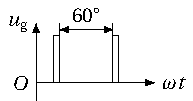
\includegraphics{figure/fig1.pdf} & (\texttt{B})~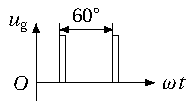
\includegraphics{figure/fig2.pdf} & (\texttt{C})~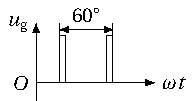
\includegraphics{figure/fig3.pdf} \end{tabular}
\end{ti}

\begin{ti}
	在大电感负载三相全控桥中,当 $\alpha = 90^\circ$ 时,整流电路的输出是\kuo{B}。
	\fourch{$U_{2}$}{$0$}{$1.414 U_{2}$}{$1.732 U_{2}$}
\end{ti}

\begin{ti}
	晶闸管触发电路中,若使控制电压 $U_{C} = 0$,改变\kuo{C}的大小,可使直流电动机负载电压 $U_{\dd} = 0$,使触发角 $\alpha = 90^\circ$。达到调定移相控制范围,实现整流、逆变的控制要求。
	\fourch{同步电压}{控制电压}{偏移电压}{锯齿波电压}
\end{ti}

\begin{ti}
	已经导通了的晶闸管可被关断的条件是流过晶闸管的电流\kuo{A}。
	\twoch{减小至维持电流 $I_{\mathrm{H}}$ 以下}{减小至擎住电流 $I_{\mathrm{L}}$ 以下}{减小至门极触发电流 $I_{\mathrm{G}}$ 以下}{减小至 \SI{5}{A} 以下}
\end{ti}

\begin{ti}
	三相全控桥式整流电路,电感性负载,控制角 $\alpha > 30^\circ$,负载电流连续,整流输出电流的平均值为 $I_{\dd}$,流过每只晶闸管的平均值电流为\kuo{B}。
	\fourch{$\frac{I_{\dd}}{2}$}{$\frac{I_{\dd}}{3}$}{$\frac{2I_{\dd}}{3}$}{$I_{\dd}$}
\end{ti}

\begin{ti}
	三相全控桥式整流电路,有一个晶闸管断路时,在一个电源周期中输出电压波形将缺少\kuo{B}波峰。
	\fourch{$1$ 个}{$2$ 个}{$3$ 个}{$4$ 个}
\end{ti}

\begin{ti}
	三相半波可控整流电路,带电阻负载,其移相范围为\kuo{C}。
	\fourch{$90^\circ$}{$120^\circ$}{$150^\circ$}{$180^\circ$}
\end{ti}

\begin{ti}
	三相全控桥式整流电路中,\kuo{B}。
	\onech{晶闸管上承受的电压是三相相电压的峰值,负载电压也是相电压}{晶闸管上承受的电压是三相线电压的峰值,负载电压也是线电压}{晶闸管上承受的电压是三相相电压的峰值,负载电压也是线电压}{晶闸管上承受的电压是三相线电压的峰值,负载电压也是相电压}
\end{ti}

\begin{ti}
	无续流二极管的三相全控桥带大电感负载时,如\kuo{C},输出电压波形会出现负值。
	\fourch{$\alpha > 0^\circ$}{$\alpha > 30^\circ$}{$\alpha > 60^\circ$}{$\alpha > 90^\circ$}
\end{ti}

\begin{ti}
	可控变流电路中,压敏电阻主要是对\kuo{C}起到保护作用。
	\fourch{晶闸管关断过电流}{电路的操作过电压}{浪涌过电压}{电压上升率过大}
\end{ti}

\begin{ti}
	过零触发电路通常应用于\kuo{C}电路中。
	\fourch{直流斩波}{可控整流}{交流调功}{交流调频}
\end{ti}

\begin{ti}
	可以用于有源逆变的电路是\kuo{D}。
	\twoch{电阻负载的半控桥}{电感负载的半控桥}{有续流二极管的全控桥}{无续流二极管的全控桥}
\end{ti}

\begin{ti}
	在晶闸管组成的直流可逆调速系统中,为使系统正常工作,其最小逆变角应选\kuo{C}。
	\fourch{$60^\circ$}{$45^\circ$}{$30^\circ$}{$15^\circ$}
\end{ti}

\begin{ti}
	两组反向并联的三相全控桥供电的直流电动机带位能性负载,当电动机在放下重物时,两组全控桥的工作状态为\kuo{D}。
	\twoch{正组整流,反组待逆变}{正组待整流,反组逆变}{正组待逆变,反组整流}{正组逆变,反组待整流}
\end{ti}

\begin{ti}
	在工业生产中,若要低电压大电流可控整流装置,常采用\kuo{D}可控整流电路。
	\twoch{三相半波}{三相全波}{三相桥式}{带平衡电抗器的双反星形}
\end{ti}

\begin{ti}
	逆变器根据直流电源的不同,分为\kuo{C}。
	\fourch{电压型和电阻型}{电流型和功率型}{电压型和电流型}{电压型和功率型}
\end{ti}

\begin{ti}
	电枢电路由两组反向并联的三相全控桥式整流电路供电的直流电动机,当正组整流桥控制角 $\alpha = 90^\circ$,反组整流桥控制角 $\alpha < 90^\circ$,则电动机处于\kuo{C}状态。
	\fourch{正反馈}{正向电动}{反相电动}{反相回馈}
\end{ti}

\begin{ti}
	三相三线交流调压电路同向不同相的晶闸管 VT\textsubscript{1},VT\textsubscript{3},VT\textsubscript{5} 的触发脉冲相位依次相差\kuo{C}。
	\fourch{$60^\circ$}{$90^\circ$}{$120^\circ$}{$180^\circ$}
\end{ti}

\begin{ti}
	变频调速中的变频器一般由\kuo{A}组成。
	\twoch{整流器、滤波器、逆变器}{放大器、滤波器、逆变器}{整流器、滤波器}{逆变器}
\end{ti}

\begin{ti}
	单相半桥(电压型)逆变器有\kuo{B}个导电臂。
	\fourch{1}{2}{3}{4}
\end{ti}

\begin{ti}
	三相半波可控整流电路,带大电感负载,移相范围为\kuo{B}。
	\fourch{$150^\circ$}{$90^\circ$}{$120^\circ$}{$180^\circ$}
\end{ti}

\begin{ti}
	三相半波可控整流电路,带大电感负载,移相范围为\kuo{B}。
	\fourch{$150^\circ$}{$90^\circ$}{$120^\circ$}{$180^\circ$}
\end{ti}

\begin{ti}
	三相全控桥式整流电路,3 号管的管压降波形中,包含有\kuo{B}两个线电压的波形。
	\fourch{$U_{\mathrm{ab}},U_{\mathrm{ac}}$}{$U_{\mathrm{ba}},U_{\mathrm{bc}}$}{$U_{\mathrm{ca}},U_{\mathrm{cb}}$}{$U_{\mathrm{ab}},U_{\mathrm{cb}}$}
\end{ti}

\begin{ti}
	在三相全控桥式整流电路中,两组三相半波电路是\kuo{B}工作的。
	\fourch{同时并联}{同时串联}{不能同时并联}{不能同时串联}
\end{ti}

\begin{ti}
	三相桥式可控整流电路中,\kuo{B}。
	\fourch{存在直流磁化问题}{不存在直流磁化问题}{不存在交流磁化问题}{存在直流磁滞问题}
\end{ti}

\begin{ti}
	三相全控桥整流电路采用单宽脉冲方案时,触发脉冲的脉宽应为\kuo{B}之间。
	\fourch{$30^\circ \sim 60^\circ$}{$60^\circ \sim 120^\circ$}{$120^\circ \sim 180^\circ$}{$30^\circ \sim 120^\circ$}
\end{ti}

\begin{ti}
	组成晶闸管触发电路的基本环节是\kuo{C}等环节。
	\twoch{同步移相、脉冲形成与整形、脉冲封锁}{同步移相、脉冲形成与整形、强触发}{同步移相、脉冲形成与整形、脉冲放大与输出}{脉冲形成与整形、双脉冲形成、脉冲放大与输出}
\end{ti}

\begin{ti}
	同步是指触发电路与主电路在\kuo{B}上有相互协调、配合的关系。
	\fourch{电压和电流}{频率和相位}{功率和阻抗角}{频率和电压的比率}
\end{ti}

\begin{ti}
	为限制 $\alpha_{\min}$ 和 $\beta_{\min}$,触发电路一般都要采取对\kuo{A}限制的措施。
	\fourch{控制电压}{同步电压}{电源电压}{偏移电压}
\end{ti}

\begin{ti}
	两组反向并联的三相全控桥供电的直流电动机,当正组控制角增大使电动机处于正向制动状态时,两组全控桥的工作状态为\kuo{B}。
	\twoch{正组整流,反组待逆变}{正组待整流,反组逆变}{正组待逆变,反组整流}{正组逆变,反组待整流}
\end{ti}

\begin{ti}
	在所有的晶闸管过电流保护措施中,最后一道保护措施是\kuo{A}。
	\fourch{快速熔断器}{过电流继电器}{直流快速开关}{脉冲移相保护}
\end{ti}

\begin{ti}
	在晶闸管斩波器中,保持晶闸管触发频率不变,改变晶闸管导通的时间从而改变直流平均电压值的控制方法叫\kuo{A}。
	\fourch{定频调宽法}{定宽调频法}{定频定宽法}{调频调宽法}
\end{ti}

\begin{ti}
	逆变器根据对无功能量的处理方法不同,可分为\kuo{C}。
	\fourch{电压型和电阻型}{电流型和功率型}{电压型和电流型}{电压型和功率型}
\end{ti}

\begin{ti}
	斩波器也可称为\kuo{C}交换。
	\fourch{AC/DC}{AC/AC}{DC/DC}{AC/AC}
\end{ti}

\begin{ti}
	三相同步变压器的相序接错,不会发生\kuo{A}的情况。
	\fourch{整流输出正常}{整流输出电压缺相}{无整流输出电压}{触发电路正常工作}
\end{ti}

\begin{ti}
	在分析晶闸管变流电路的波形时,控制角的大小是按下述\kuo{B}方法计算的。
	\onech{不论整流电路还是逆变电路,都是从交流电压过零点开始向右计算}{不论整流电路还是逆变电路,都是从自然换相点开始向右计算}{整流电路从自然换相点开始向右计算,逆变电路从自然换相点开始向左计算}{整流电路从自然换相点开始向左计算,逆变电路从自然换相点开始向右计算}
\end{ti}

\begin{ti}
	三相半波可控整流电路,带电阻负载,其输出直流电压的波形在\kuo{D}内是连续的。
	\twoch{$90^\circ$}{$120^\circ$}{$150^\circ$}{不一定,与电路是否有续流二极管等情况有关}
\end{ti}

\begin{ti}
	三相全控桥式整流电路,带电感负载,晶闸管的导通规律是\kuo{B}。
	\twoch{每隔 $120^\circ$ 换相一次,每只管子导通 $60^\circ$}{每隔 $60^\circ$ 换相一次,每只管子导通 $120^\circ$}{同一相中两只管子的触发脉冲相隔 $120^\circ$}{同一组中相邻两只管子的触发脉冲相隔 $60^\circ$}
\end{ti}

\begin{ti}
	三相桥式半控整流电路带电感性负载加上续流二极管是为了\kuo{D}。
	\twoch{增大输出直流平均电压}{减少输出直流平均电压}{防止晶闸管不能导通}{防止晶闸管不能关断}
\end{ti}

\begin{ti}
	无续流二极管的三相全控桥带大电感负载时,如\kuo{C},输出电压波形会出现负值。
	\fourch{$\alpha > 0^\circ$}{$\alpha > 30^\circ$}{$\alpha > 60^\circ$}{$\alpha > 90^\circ$}
\end{ti}

\begin{ti}
	晶闸管触发电路的触发脉冲波形一般不采用\kuo{D}波形。
	\fourch{矩形脉冲}{强触发脉冲}{脉冲列}{锯齿波}
\end{ti}

\begin{ti}
	在晶闸管触可控整流电路所用的触发电路中,控制角的改变通常是以\kuo{D}的方式来实现的。
	\fourch{改变同步信号的大小}{改变电源电压的大小}{改变偏移电源的大小}{改变控制电压的大小}
\end{ti}

\begin{ti}
	晶闸管触相控整流电路采用\kuo{B}电路。
	\fourch{过零触发}{移相触发}{同步触发}{计数触发}
\end{ti}

\begin{ti}
	脉冲变压器传递的是\kuo{A}。
	\twoch{前沿陡峭、顶部平坦的矩形信号}{正弦波电压信号}{能量的变换}{电压的变换}
\end{ti}

\begin{ti}
	两组反向并联的三相全控桥供电的直流电动机,当正组控制角增大使电动机处于正向制动状态时,两组全控桥的工作状态为\kuo{B}。
	\twoch{正组整流,反组待逆变}{正组待整流,反组逆变}{正组待逆变,反组整流}{正组逆变,反组待整流}
\end{ti}

\begin{ti}
	以下\kuo{B}情况不属于有源逆变。
	\twoch{直流可逆拖动系统}{晶闸管中频电源}{绕线异步电动机串级调速系统}{高压直流输电}
\end{ti}

\begin{ti}
	电压型逆变器的直流端\kuo{D}。
	\fourch{串联大电感}{串联大电容}{并联大电感}{并联大电容}
\end{ti}

\begin{ti}
	在晶闸管可逆调速系统中,为防止逆变颠覆,应设置\kuo{C}保护环节。
	\fourch{限制 $\alpha_{\min}$}{限制 $\beta_{\min}$}{限制 $\alpha_{\min}$ 和 $\beta_{\min}$}{限制 $\beta_{\max}$}
\end{ti}

\begin{ti}
	三相三线交流调压电路同相不同向的晶闸管 VT\textsubscript{1},VT\textsubscript{4} 的触发脉冲相位依次相差\kuo{D}。
	\fourch{$60^\circ$}{$90^\circ$}{$120^\circ$}{$180^\circ$}
\end{ti}

\begin{ti}
	单相半桥(电压型)逆变器的输出电压为\kuo{B}。
	\fourch{正弦波}{矩形波}{锯齿波}{尖顶波}
\end{ti}

\begin{ti}
	在并联谐振式晶闸管逆变器中,为求得较高的功率因数和效率,应使晶闸管触发脉冲的频率\kuo{C}负载电路的谐振频率。
	\fourch{远大于}{大于}{接近于}{小于}
\end{ti}

\begin{ti}
	晶闸管在导通状态下,管耗等于管子两端电压乘以\kuo{A}。
	\twoch{阳极电流}{门极电流}{阳极电流与门极电流之和}{阳极电流与门极电流之差}
\end{ti}

\begin{ti}
	电力晶体管(GTR)是一种\kuo{A}结构的半导体器件。
	\fourch{四层三端}{五层三端}{三层二端}{三层三端}
\end{ti}

\begin{ti}
	单相半波可控整流电路,阻性负载,导通角 $\theta$ 的最大变化范围是 $0^\circ \sim $ \kuo{D}。
	\fourch{$90^\circ$}{$120^\circ$}{$150^\circ$}{$180^\circ$}
\end{ti}

\begin{ti}
	三相半波可控整流电路,阻性负载,导通角 $\theta$ 的最大变化范围是 $0^\circ \sim $ \kuo{C}。
	\fourch{$90^\circ$}{$120^\circ$}{$150^\circ$}{$180^\circ$}
\end{ti}

\begin{ti}
	三相全控桥式整流电路,阻性负载,控制角 $\alpha$ 的最大移相范围是 $0^\circ \sim $ \kuo{B}。
	\fourch{$90^\circ$}{$120^\circ$}{$150^\circ$}{$180^\circ$}
\end{ti}

\begin{ti}
	三相半波可控整流电路电源电压波形的自然换向点比单相半波可控整流电路的自然换向点\kuo{B}。
	\fourch{超前 $30^\circ$}{滞后 $30^\circ$}{超前 $60^\circ$}{滞后 $60^\circ$}
\end{ti}

\begin{ti}
	单相全波可控整流电路,电感性负载,控制角 $\alpha \leq 30^\circ$,每个周期内输出电压的平均值为\kuo{B}。
	\fourch{$U_{\dd} = 0.45 U_{2} \cos\alpha$}{$U_{\dd} = 0.9 U_{2} \cos\alpha$}{$U_{\dd} = 1.17 U_{2} \cos\alpha$}{$U_{\dd} = 2.34 U_{2} \cos\alpha$}
\end{ti}

\begin{ti}
	三相全控桥式整流电路,电感性负载,控制角 $\alpha > 30^\circ$,负载电流连续,整流输出电流的平均值为 $I_{\dd}$,流过每只晶闸管的平均值电流为\kuo{B}。
	\fourch{$\frac{I_{\dd}}{2}$}{$\frac{I_{d}}{3}$}{$\frac{2I_{\dd}}{3}$}{$I_{\dd}$}
\end{ti}

\begin{ti}
	单相全控桥式有源逆变电路最小逆变角 $\beta$ 为\kuo{D}。
	\fourch{$1^\circ \sim 3^\circ$}{$10^\circ \sim 15^\circ$}{$20^\circ \sim 25^\circ$}{$30^\circ \sim 35^\circ$}
\end{ti}

\begin{ti}
	三相全控制桥式有源逆变电路,在交流电源一个周期里,输出电压脉动\kuo{D}次。
	\fourch{2}{3}{4}{6}
\end{ti}

\begin{ti}
	有源逆变电路是\kuo{B}。
	\fourch{AC/DC 变换器}{DC/AC 变换器}{AC/AC 变换器}{DC/DC 变换器}
\end{ti}

\begin{ti}
	PWM 脉宽调制技术用于\kuo{B}。
	\fourch{有源逆变器}{无源逆变器}{脉冲触发器}{脉冲移相器}
\end{ti}

\begin{ti}
	KC04 型集成触发电路引角 1 和 15 输出两个互差 $180^\circ$ 的触发脉冲,经过放大隔离后,可驱动三相全控桥\kuo{A}的两只晶闸管。
	\fourch{同一桥臂}{不同桥臂}{共阴组}{共阳组}
\end{ti}

\begin{ti}
	三相全控桥式整流电路,有一个晶闸管断路时,在一个电源周期中输出电压波形将缺少\kuo{B}波峰。
	\fourch{1 个}{2 个}{3 个}{4个}
\end{ti}

\begin{ti}
	集成触发电路中 KC41C 集成电路芯片被称为\kuo{B}。
	\fourch{集成移相触发器}{六路双脉形成器}{脉冲同步器}{脉冲信号发生器}
\end{ti}

\begin{ti}
	已经导通了的晶闸管可被关断的条件是流过晶闸管的电流\kuo{B}。
	\twoch{减小至维持电流 $I_{\mathrm{H}}$ 以下}{减小至擎住电流 $I_{\mathrm{L}}$ 以下}{减小至门极触发电流 $I_{\mathrm{G}}$ 以下}{减小至 \SI{5}{A} 以下}
\end{ti}

\begin{ti}
	对于同一晶闸管,维持电流 $I_{\HH}$ 与擎住电流 $I_{\LL}$ 的关系是\kuo{A}。
	\fourch{$I_{\HH} \approx (2 \sim 4) I_{\LL}$}{$I_{\LL} \approx (2 \sim 4) I_{\HH}$}{$I_{\HH} = I_{\LL}$}{$I_{\HH} \geq I_{\LL}$}
\end{ti}

\begin{ti}
	单相半波可控整流电路中,晶闸管可能承受的反向峰值电压为\kuo{B}。
	\fourch{$U_{2}$}{$\sqrt{2}U_{2}$}{$2\sqrt{2}U_{2}$}{$\sqrt{6}U_{2}$}
\end{ti}

\begin{ti}
	单相半控桥电感性负载电路中,在负载两端并联一个续流二极管的目的是\kuo{D}。
	\twoch{增加晶闸管的导电能力}{抑制温漂}{增加输出电压稳定性}{防止失控现象的产生}
\end{ti}

\begin{ti}
	电阻性负载三相半波可控整流电路,控制角 $\alpha$ 的范围是\kuo{D}。
	\fourch{$30^\circ \sim 150^\circ$}{$0^\circ \sim 120^\circ$}{$15^\circ \sim 125^\circ$}{$0^\circ \sim 150^\circ$}
\end{ti}

\begin{ti}
	三相全控桥式变流电路工作于有源逆变状态,输出电压平均值 $U_{\dd}$ 的表达式是\kuo{A}。
	\fourch{$U_{\dd} = -2.34 U_{2} \cos\beta$}{$U_{\dd} = 1.17 U_{2} \cos\beta$}{$U_{\dd} = 2.34 U_{2} \cos\beta$}{$U_{\dd} = -0.9 U_{2} \cos\beta$}
\end{ti}

\begin{ti}
	可在第二象限工作交流电路是\kuo{C}。
	\twoch{单相全控桥}{单相半控桥}{单相反并联(双重)全控桥}{三相半波可控变流电路}
\end{ti}

\begin{ti}
	在高压直流输电系统中,变流器 1 和变流器 2 中间的直流环节起着功率传输作用,控制功率流向的方法是\kuo{D}。
	\onech{调节变流器 1 侧变压器}{调节变流器 2 侧变压器}{同时调节两侧变压器}{调节变流器 1 和变流器 2 的 $U_{\dd 1}$、$U_{\dd 2}$ 的极性和大小}
\end{ti}

\begin{ti}
	SPWM 逆变器有两种调制方式:双极性和\kuo{A}。
	\fourch{单极性}{多极性}{三极性}{四极性}
\end{ti}

\begin{ti}
	对于移相控制电路,为了限制最小移相控制角和设置移相范围,可在输入控制信号的输入控制信号的输入端再叠加一个\kuo{B}。
	\fourch{交流电压}{偏移电压}{同步信号}{触发信号}
\end{ti}

\begin{ti}
	KC04 型集成触发电路的引脚 1 和 15 输出的触发脉冲是两个相位互差 $180^\circ$ \kuo{C}。
	\fourch{负脉冲}{正脉冲}{双脉冲}{尖峰脉冲}
\end{ti}

\begin{ti}
	降压斩波电路中,已知电源电压 $U_{\dd} = \SI{16}{V}$,负载电压 $U_{\oo} = \SI{12}{V}$,斩波周期 $T = \SI{4}{ms}$,则开通时间 $T_{\mathrm{ab}} = $ \kuo{C}。
	\fourch{\SI{1}{ms}}{\SI{2}{ms}}{\SI{3}{ms}}{\SI{4}{ms}}
\end{ti}

\begin{ti}
	可以用于有源逆变的电路是\kuo{D}。
	\twoch{电阻负载的半控桥}{电感负载的半控桥}{有续流二极管的全控桥}{无续流二极管的全控桥}
\end{ti}

\begin{ti}
	两组反向并联的三相全控桥供电的直流电动机带位能性负载,当电动机在放下重物时,两组全控桥的工作状态为\kuo{D}。
	\twoch{正组整流,反组待逆变}{正组待整流,反组逆变}{正组待逆变,反组整流}{正组逆变,反组待整流}
\end{ti}

\begin{ti}
	三相三线交流调压电路同向不同相的晶闸管 VT\textsubscript{1},VT\textsubscript{3},VT\textsubscript{5} 的触发脉冲相位依次相差\kuo{C}。
	\fourch{$60^\circ$}{$90^\circ$}{$120^\circ$}{$180^\circ$}
\end{ti}

\begin{ti}
	将直流电能转换为交流电能馈送给交流电网的变流器是\kuo{A}。
	\fourch{有源逆变器}{A/D 变换器}{D/A 变换器}{无源逆变器}
\end{ti}

\begin{ti}
	三相全控桥式整流电路中,共阳极组的三只晶闸管的触发脉冲相位互差\kuo{C}。
	\fourch{$60^\circ$}{$90^\circ$}{$120^\circ$}{$150^\circ$}
\end{ti}

\begin{ti}
	晶闸管的三个引出电极分别是\kuo{A}。
	\twoch{阳极、阴极、门极}{阳极、阴极、栅极}{栅极、漏极、源极}{发射极、基极、集电极}
\end{ti}

\begin{ti}
	单相半波可控整流带电阻性负载 $R$ 电路,设变压器二次侧相电压有效值为 $U_{2}$,则直流电流平均值为\kuo{A}。
	\fourch{$0.45 \frac{U_{2}}{R} (1 + \cos\alpha)$}{$0.225 \frac{U_{2}}{R} (1 + \cos\alpha)$}{$0.9 \frac{U_{2}}{R} (1 + \cos\alpha)$}{$0.45 \frac{U_{2}}{R} \bigl( \frac{1 - \cos\alpha}{2} \bigr)$}
\end{ti}

\begin{ti}
	三相全控桥式整流电路中同一相上、下两只晶闸管触发脉冲相位差\kuo{D}度。
	\fourch{60}{90}{120}{180}
\end{ti}

\begin{ti}
	单相半控桥式无续流二极管整流电路输出电压平均值为\kuo{A},设变压器二次侧相电压有效值为 $U_{2}$。
	\fourch{$0.9 U_{2} \frac{1 + \cos\alpha}{2}$}{$0.9 U_{2} \times \sqrt{2} \frac{1 + \cos\alpha}{2}$}{$0.5 U_{2} (1 + \cos\alpha)$}{$0.9 U_{2} \frac{1 - \cos\alpha}{2}$}
\end{ti}

\begin{ti}
	三相半控桥式整流电路(共阴极组)要求触发脉冲发\kuo{C}度间隔触发。
	\fourch{60}{90}{120}{180}
\end{ti}

\begin{ti}
	当晶闸管承受反向阳极电压且门极施加正向脉冲时,正常情况下晶闸管都将工作在\kuo{B}。
	\fourch{导通状态}{关断状态}{饱和状态}{不定}
\end{ti}

\begin{ti}
	在直流降压斩波电路中,电源电压 $U_{\dd}$ 与负载电压平均值 $U_{\oo}$ 之间的关系是\kuo{B},设开关周期和开关导通时间分别为 $T$、$T_{\mathrm{on}}$。
	\fourch{$U_{\oo} = \frac{T_{\mathrm{on}}}{T} U_{\dd}$}{$U_{\dd} = \frac{T_{\mathrm{on}}}{T} U_{\oo}$}{$U_{\oo} = \frac{T}{T_{\mathrm{on}}} U_{\dd}$}{$U_{\dd} = \frac{T}{T_{\mathrm{on}}} U_{\oo}$}
\end{ti}

\begin{ti}
	三相半波可控电阻性负载电路中,晶闸管可能承受的最大正向电压为\kuo{D},设 $U_{2}$ 为变压器二次侧相电压有效值。
	\fourch{$\frac{\sqrt{2}}{2} U_{2}$}{$\sqrt{2} U_{2}$}{$2 U_{2}$}{$\sqrt{6} U_{2}$}
\end{ti}

\begin{ti}
	在型号为 KP10-12G 中,数字 10 表示\kuo{B}。
	\fourch{额定电压 \SI{10}{V}}{额定电流 \SI{10}{A}}{额定电压 \SI{1000}{V}}{额定电流 \SI{1000}{A}}
\end{ti}

\begin{ti}
	下列电路中,不可以实现有源逆变的有\kuo{B}。
	\twoch{三相半波可控整流电路}{三相桥式半控整流电路}{单相桥式可控整流电路}{单相全波可控整流电路}
\end{ti}

\begin{ti}
	整流变压器漏抗对电路的影响有\kuo{C}。
	\twoch{整流装置的功率因数降低}{输出电压脉动减小}{电流变化缓和}{引起相间短路}
\end{ti}

\begin{ti}
	功率晶体管 GTR 从高电压小电流向低电压大电流跃变的现象称为\kuo{B}。
	\fourch{一次击穿}{二次击穿}{临界饱和}{反向截止}
\end{ti}

\begin{ti}
	逆导晶闸管是将大功率二极管与何种器件集成在一个管芯上而成\kuo{B}。
	\fourch{大功率三极管}{逆阻型晶闸管}{双向晶闸管}{可关断晶闸管}
\end{ti}

\begin{ti}
	已经导通了的晶闸管可被关断的条件是流过晶闸管的电流\kuo{B}。
	\twoch{减小至维持电流 $I_{\HH}$ 以下}{减小至擎住电流 $I_{\LL}$ 以下}{减小至门极触发电流 $I_{\GG}$ 以下}{减小至 \SI{5}{A} 以下}
\end{ti}

\begin{ti}
	单相半波可控整流电路中,晶闸管可能承受的反向峰值电压为\kuo{B}。
	\fourch{$U_{2}$}{$\sqrt{2}U_{2}$}{$2\sqrt{2}U_{2}$}{$\sqrt{6}U_{2}$}
\end{ti}

\begin{ti}
	单相半控桥电感性负载电路中,在负载两端并联一个续流二极管的目的是\kuo{D}。
	\twoch{增加晶闸管的导电能力}{抑制温漂}{增加输出电压稳定性}{防止失控现象的产生}
\end{ti}

\begin{ti}
	三相全控桥式变流电路工作于有源逆变状态,输出电压平均值 $U_{\dd}$ 的表达式是\kuo{A}。
	\fourch{$U_{\dd} = - 2.34 U_{2} \cos\beta$}{$U_{\dd} = 1.17 U_{2} \cos\beta$}{$U_{\dd} = 2.34 U_{2} \cos\beta$}{$U_{\dd} = - 0.9 U_{2} \cos\beta$}
\end{ti}

\begin{ti}
	若减小 SPWM 逆变器输出电压基波幅值,可采用的控制方法是\kuo{C}。
	\twoch{减小三角波频率}{减小三角波幅度}{减小输入正弦控制电压幅值}{减小输入正弦控制电压频率}
\end{ti}

\begin{ti}
	当晶闸管承受反向阳极电压时,不论门极加何种极性触发电压,管子都将工作在\kuo{B}。
	\fourch{导通状态}{关断状态}{饱和状态}{不定}
\end{ti}

\begin{ti}
	单相半波可控整流电阻性负载电路中,控制角 $\alpha$ 的最大移相范围是\kuo{D}。
	\fourch{$90^\circ$}{$120^\circ$}{$150^\circ$}{$180^\circ$}
\end{ti}

\begin{ti}
	单相全控桥式整流大电感负载电路中,控制角 $\alpha$ 的移相范围是\kuo{A}。
	\fourch{$0^\circ \sim 90^\circ$}{$0^\circ \sim 180^\circ$}{$90^\circ \sim 180^\circ$}{$180^\circ \sim 360^\circ$}
\end{ti}

\begin{ti}
	在大电感负载三相全控桥中,当 $\alpha = 90^\circ$ 时,整流电路的输出是\kuo{B}.
	\fourch{$U_{2}$}{$0$}{$1.414 U_{2}$}{$1.732 U_{2}$}
\end{ti}

\begin{ti}
	三相半波可控整流电路的自然换相点是\kuo{B}。
	\twoch{交流相电压的过零点}{本相相电压与相邻相电压正半周的交点处}{比三相不控整流电路的自然换相点超前 $30^\circ$}{比三相不控整流电路的自然换相点滞后 $60^\circ$}
\end{ti}

\begin{ti}
	单相半波可控整流电路,阻性负载,导通角 $\theta$ 的最大变化范围是 $0^\circ \sim$ \kuo{D}。
	\fourch{$90^\circ$}{$120^\circ$}{$150^\circ$}{$180^\circ$}
\end{ti}

\begin{ti}
	三相全控桥式整流电路,有一个晶闸管断路时,在一个电源周期中输出电压波形将缺少\kuo{B}波峰。
	\fourch{1 个}{2 个}{3 个}{4 个}
\end{ti}

\begin{ti}
	为了减小门极损耗,晶闸管正常导通的方法是阳极加正向电压,门极加\kuo{A}。
	\fourch{正脉冲}{负脉冲}{直流}{正弦波}
\end{ti}

\begin{ti}
	三相半波可控整流电路电源电压波形的自然换向点比单相半波可控整流电路的自然换向点\kuo{B}。
	\fourch{超前 $30^\circ$}{滞后 $30^\circ$}{超前 $60^\circ$}{滞后 $60^\circ$}
\end{ti}

\begin{ti}
	单相全波可控整流电路,电感性负载,控制角 $\alpha \leq 30^\circ$,每个周期内输出电压的平均值为\kuo{B}。
	\fourch{$U_{\dd} = 0.45 U_{2} \cos\alpha$}{$U_{\dd} = 0.9 U_{2} \cos\alpha$}{$U_{\dd} = 1.17 U_{2} \cos\alpha$}{$U_{\dd} = 2.34 U_{2} \cos\alpha$}
\end{ti}

\begin{ti}
	单相全控桥,带反电动势负载,当控制角 $\alpha$ 大于不导电角 $\delta$ 时,晶闸管的导通角 $\theta$ 为\kuo{A}。
	\fourch{$\uppi - \alpha - \delta$}{$\uppi - \alpha + \delta$}{$\uppi - 2\alpha$}{$\uppi - 2\delta$}
\end{ti}

\begin{ti}
	集成触发电路中 KC41C 集成电路芯片被称为\kuo{B}。
	\fourch{集成移相触发器}{六路双脉形成器}{脉冲同步器}{脉冲信号发生器}
\end{ti}

\begin{ti}
	三相全控制桥式有源逆变电路,在交流电源一个周期里,输出电压脉动\kuo{D}次。
	\fourch{2}{3}{4}{6}
\end{ti}

\begin{ti}
	下列器件中为全控型器件的是\kuo{D}。
	\fourch{双向晶闸管}{快速晶闸管}{光控晶闸管}{功率场效应晶体管}
\end{ti}

\begin{ti}
	KC04 型集成触发电路引角 1 和 15 输出两个互差 $180^\circ$ 的触发脉冲,经过放大隔离后,可驱动三相全控桥\kuo{A}的两只晶闸管。
	\fourch{同一桥臂}{不同桥臂}{共阴组}{共阳组}
\end{ti}

\begin{ti}
	单相半控桥整流电路的两只晶闸管的触发脉冲依次应相差\kuo{A}度。
	\fourch{$180^\circ$}{$60^\circ$}{$360^\circ$}{$120^\circ$}
\end{ti}

\begin{ti}
	三相交流调压电路 $60^\circ < \alpha < 90^\circ$ 时晶闸管的导通情况\kuo{B}。
	\fourch{一个}{两个}{三个}{两个或三个}
\end{ti}

\begin{ti}
	大电感性负载的三相半波整流电路,流过晶闸管的平均电流为\kuo{B}。
	\fourch{$\frac{1}{2}I_{\dd}$}{$\frac{1}{3}I_{\dd}$}{$\frac{\sqrt{2}}{2}I_{\dd}$}{$\frac{\sqrt{3}}{3}I_{\dd}$}
\end{ti}

\begin{ti}
	$\alpha$ 为\kuo{C}度时,三相半波可控整流电路,电阻性负载输出的电压波形,处于连续和断续的临界状态。
	\fourch{$0^\circ$}{$60^\circ$}{$30^\circ$}{$120^\circ$}
\end{ti}

\begin{ti}
	晶闸管触发电路中,若改变\kuo{B}的大小,则输出脉冲产生相位移动,达到移相控制的目的。
	\fourch{同步电压}{控制电压}{脉冲变压器变比}{锯齿波电压}
\end{ti}

\begin{ti}
	单相交流调压电路,输出电压最大值,$\alpha$ 为\kuo{A}。
	\fourch{$0^\circ$}{$60^\circ$}{$90^\circ$}{$180^\circ$}
\end{ti}

\begin{ti}
	可实现有源逆变的电路为\kuo{A}。
	\twoch{三相半波可控整流电路}{三相半控桥整流桥电路}{单相全控桥接续流二极管电路}{单相半控桥整流电路}
\end{ti}

\begin{ti}
	单相半控桥,带大电感负载,直流侧并联续流管的主要作用是\kuo{A}。
	\twoch{防止失控现象}{减小输出电压的脉动}{减小输出电流的脉动}{直流侧过电压保护}
\end{ti}

\begin{ti}
	三相全控桥式整流电路,有一个晶闸管断路时,在一个电源周期中输出电压波形将缺少\kuo{B}波峰。
	\fourch{1 个}{2 个}{3 个}{4 个}
\end{ti}

\begin{ti}
	在一般可逆电路中,最小逆变角 $\beta_{\min}$ 选在下面那一种范围合理\kuo{A}。
	\fourch{$30^\circ \sim 35^\circ$}{$10^\circ \sim 15^\circ$}{$0^\circ \sim 10^\circ$}{$0^\circ$}
\end{ti}

\begin{ti}
	三相桥式半控整流电路中,要求共阴极组晶闸管的触发脉冲之间相位差为\kuo{B}。
	\fourch{$60^\circ$}{$120^\circ$}{$150^\circ$}{$180^\circ$}
\end{ti}

\begin{ti}
	三相可逆晶闸管变流器的触发电路至少应能达到\kuo{B}的移相范围。
	\fourch{$90^\circ$}{$180^\circ$}{$240^\circ$}{$300^\circ$}
\end{ti}

\begin{ti}
	逆变器的任务是把\kuo{B}。
	\fourch{交流电变直流电}{直流电变交流电}{交流电变交流电}{直流电变直流电}
\end{ti}

\begin{ti}
	电压型逆变器的直流端\kuo{D}。
	\fourch{串联大电感}{串联大电容}{并联大电感}{并联大电容}
\end{ti}

\begin{ti}
	单相半桥(电压型)逆变器的直流端接有两个相互串联的\kuo{A}。
	\fourch{容量足够大的电容}{大电感}{容量足够小的电容}{小电感}
\end{ti}

\begin{ti}
	直流电动机用斩波器进行调速时,可实现\kuo{B}。
	\fourch{有级调速}{无级调速}{恒定转速}{分档调速}
\end{ti}

\begin{ti}
	直流电动机所用的斩波器主要起\kuo{D}作用。
	\fourch{调电阻}{调电流}{调电抗}{调电压}
\end{ti}

\begin{ti}
	电力晶体管 GTR 内部电流是由\kuo{C}形成的。
	\fourch{电子}{空穴}{电子和空穴}{有电子但无空穴}
\end{ti}

\begin{ti}
	绝缘双极晶体管的开关速度\kuo{B}电力场效应管。
	\fourch{稍高于}{低于}{等于}{远高于}
\end{ti}

\begin{ti}
	在电力电子装置中,电力晶体管 GTR 一般工作在\kuo{D}状态。
	\fourch{放大}{截止}{饱和}{开关}
\end{ti}

\begin{ti}
	绝缘双极晶体管的内部为\kuo{D}层结构。
	\fourch{1}{2}{3}{4}
\end{ti}

\begin{ti}
	双向晶闸管额定电流采用\kuo{B}。
	\fourch{平均值}{有效值}{瞬时值}{峰值}
\end{ti}

\begin{ti}
	三相三线交流调压电路同向不同相的晶闸管 VT\textsubscript{1}、VT\textsubscript{3}、VT\textsubscript{5} 的触发脉冲相位依次相差\kuo{C}。
	\fourch{$60^\circ$}{$90^\circ$}{$120^\circ$}{$180^\circ$}
\end{ti}

\begin{ti}
	电力晶体管在使用时,要防止\kuo{A}。
	\fourch{二次击穿}{雷电击穿}{时间久而失效}{工作在开关状态}
\end{ti}

\begin{ti}
	同步电动机晶闸管励磁装置主电路采用三相桥式全控整流电路时,晶闸管 VT\textsubscript{1}、VT\textsubscript{3}、VT\textsubscript{5} 的触发脉冲互相相隔\kuo{C}。
	\fourch{$60^\circ$}{$90^\circ$}{$120^\circ$}{$180^\circ$}
\end{ti}

\begin{ti}
	三相全控桥的六个晶闸管上的触发脉冲依次相差\kuo{B}.
	\fourch{$30^\circ$}{$60^\circ$}{$90^\circ$}{$120^\circ$}
\end{ti}

\begin{ti}
	在晶闸管上组成的可逆调速系统,为使系统正常工作,其最少逆变角 $\beta_{\min}$ 一般选\kuo{C}。
	\fourch{$60^\circ$}{$45^\circ$}{$30^\circ$}{$15^\circ$}
\end{ti}

\begin{ti}
	晶闸管逆变器输出交流电的频率由\kuo{D}来决定。
	\twoch{一组晶闸管的导通时间}{两组组晶闸管的导通时间}{一组晶闸管的触发脉冲频率}{两组晶闸管的触发脉冲频率}
\end{ti}

\begin{ti}
	单相半桥(电压型)逆变器的每个导电臂由一个电力晶体管和一个\kuo{D}的二极管组成。
	\fourch{串联}{反串联}{并联}{反并联}
\end{ti}

\begin{ti}
	直流电动机用斩波器进行调速时,当电压降低后,机械特性硬度\kuo{C}。
	\fourch{变软}{变硬}{不变}{不定}
\end{ti}

\begin{ti}
	电力场效应管 MOSFET 是理想的\kuo{A}控制器件。
	\fourch{电压}{电流}{电阻}{功率}
\end{ti}

\begin{ti}
	要使绝缘双极晶体管导通,应\kuo{A}。
	\fourch{在栅极加正电压}{在集电极加正电压}{在栅极加负电压}{在集电极加负电压}
\end{ti}

\begin{ti}
	电力晶体管 GTR 有\kuo{B}个 PN 结。
	\fourch{1}{2}{3}{4}
\end{ti}

\begin{ti}
	功率场效应管的三个引脚符号为\kuo{D}。
	\twoch{源极 S、漏极 D、发射极 E}{漏极 D、发射极 E、集电极 C}{栅极 G、发射极 E、集电极 C}{源极 S、漏极 D、栅极 G}
\end{ti}

\begin{ti}
	电力晶体管的缺点是\kuo{D}。
	\twoch{功率容量小}{必须具备专门的强迫换流电路}{具有线性放大特性}{易受二次击穿而损坏}
\end{ti}

\begin{ti}
	大电感性负载的三相半波整流电路,流过晶闸管的平均电流为:\kuo{B}。
	\fourch{$\frac{1}{2}I_{\dd}$}{$\frac{1}{3}I_{\dd}$}{$\frac{\sqrt{2}}{2}I_{\dd}$}{$\frac{\sqrt{3}}{3}I_{\dd}$}
\end{ti}

\begin{ti}
	单相交流调压电路,输出电压最大值,$\alpha$ 为:\kuo{A}。
	\fourch{$0^\circ$}{$60^\circ$}{$90^\circ$}{$180^\circ$}
\end{ti}

\begin{ti}
	晶闸管在导通状态下,管耗等于管子两端电压乘以\kuo{A}。
	\twoch{阳极电流}{门极电流}{阳极电流与门极电流之和}{阳极电流与门极电流之差}
\end{ti}

\begin{ti}
	电力晶体管(GTR)是一种\kuo{A}结构的半导体器件。
	\fourch{四层三端}{五层三端}{三层二端}{三层三端}
\end{ti}

\begin{ti}
	单相半波可控整流电路,阻性负载,导通角 $\theta$ 的最大变化范围是 $0^\circ \sim $\kuo{D}。
	\fourch{$90^\circ$}{$120^\circ$}{$150^\circ$}{$180^\circ$}
\end{ti}

\begin{ti}
	大功率电力晶体管 GTR 在逆变电路中是用来作为开关器件的,其工作过程总是在\kuo{D}之间进行交替的。
	\twoch{放大状态和饱和状态}{饱和状态和低阻状态}{放大状态和截止状态}{饱和状态和截止状态}
\end{ti}

\begin{ti}
	电力场效应管 MOSFET\kuo{B}现象。
	\fourch{有二次击穿}{无二次击穿}{要防止二次击穿}{无静电击穿}
\end{ti}

\begin{ti}
	电力场效应管适应于\kuo{C}的设备。
	\fourch{高速、大容量}{低速、大容量}{高速、小容量}{低速、小容量}
\end{ti}

\begin{ti}
	在工业生产中,若要低电压大电流可控整流装置,常采用\kuo{D}可控整流电路。
	\twoch{三相半波}{三相全波}{三相桥式}{带平衡电抗器的双反星形}
\end{ti}

\begin{ti}
	单相半波可控整流电路中,晶闸管可能承受的反向峰值电压为\kuo{B}。
	\fourch{$U_{2}$}{$\sqrt{2} U_{2}$}{$2\sqrt{2} U_{2}$}{$\sqrt{6} U_{2}$}
\end{ti}

\begin{ti}
	单相半控桥电感性负载电路中,在负载两端并联一个续流二极管的目的是\kuo{D}。
	\twoch{增加晶闸管的导电能力}{抑制温漂}{增加输出电压稳定性}{防止失控现象的产生}
\end{ti}

\begin{ti}
	三相全控桥式变流电路工作于有源逆变状态,处于关断状态的晶闸管承受的的反向电压的期间角为\kuo{C}。
	\fourch{$120^\circ$}{$120^\circ - \beta$}{$180^\circ - \beta$}{$\beta$}
\end{ti}

\begin{ti}
	三相全控桥式变流电路工作于有源逆变状态,输出电压平均值 $U_{\dd}$ 的表达式是\kuo{A}。
	\fourch{$U_{\dd} = -2.34 U_{2} \cos\beta$}{$U_{\dd} = 1.17 U_{2} \cos\beta$}{$U_{\dd} = 2.34 U_{2} \cos\beta$}{$U_{\dd} = -0.9 U_{2} \cos\beta$}
\end{ti}

\begin{ti}
	对于移相控制电路,为了限制最小移相控制角和设置移相范围,可在输入控制信号的输入控制信号的输入端再叠加一个\kuo{B}。
	\fourch{交流电压}{偏移电压}{同步信号}{触发信号}
\end{ti}

\begin{ti}
	在大电感负载三相全控桥中,当 $\alpha = 90^\circ$ 时,整流电路的输出是\kuo{B}。
	\fourch{$U_{2}$}{$0$}{$1.414 U_{2}$}{$1.732 U_{2}$}
\end{ti}

\begin{ti}
	在型号为 KP10-12G 中,数字 10 表示\kuo{B}。
	\fourch{额定电压 \SI{10}{V}}{额定电流 \SI{10}{A}}{额定电压 \SI{1000}{V}}{额定电流 \SI{1000}{A}}
\end{ti}

\begin{ti}
	下列电路中,不可以实现有源逆变的有\kuo{B}。
	\twoch{三相半波可控整流电路}{三相桥式半控整流电路}{单相桥式可控整流电路}{单相全波可控整流电路}
\end{ti}

\begin{ti}
	单相全控桥反电动势负载电路中,当控制角 $\alpha$ 大于不导电角 $\delta$ 时,晶闸管的导通角 $\theta = $\kuo{C}。
	\fourch{$\uppi - \alpha$}{$\uppi + \alpha$}{$\uppi - \delta - \alpha$}{$\uppi + \delta - \alpha$}
\end{ti}

\begin{ti}
	功率晶体管 GTR 从高电压小电流向低电压大电流跃变的现象称为\kuo{B}。
	\fourch{一次击穿}{二次击穿}{临界饱和}{反向截止}
\end{ti}

\begin{ti}
	逆导晶闸管是将大功率二极管与何种器件集成在一个管芯上而成\kuo{B}。
	\fourch{大功率三极管}{逆阻型晶闸管}{双向晶闸管}{可关断晶闸管}
\end{ti}

\begin{ti}
	已经导通了的晶闸管可被关断的条件是流过晶闸管的电流\kuo{A}。
	\twoch{减小至维持电流 $I_{\HH}$ 以下}{减小至擎住电流 $I_{\LL}$ 以下}{减小至门极触发电流 $I_{\GG}$ 以下}{减小至 \SI{5}{A} 以下}
\end{ti}

\begin{ti}
	单相半波整流电路中,晶闸管可能承受的反向峰值电压为\kuo{B}。
	\fourch{$U_{2}$}{$\sqrt{2} U_{2}$}{$2\sqrt{2} U_{2}$}{$\sqrt{6} U_{2}$}
\end{ti}

\begin{ti}
	单相半控桥电感性负载电路中,在负载两端并联一个续流二极管的目的是\kuo{D}。
	\twoch{增加晶闸管的导电能力}{抑制温漂}{增加输出电压稳定性}{防止失控现象的产生}
\end{ti}

\begin{ti}
	三相全控桥式变流电路工作于有源逆变状态,输出电压平均值 $U_{\dd}$ 的表达式是\kuo{A}。
	\fourch{$U_{\dd} = -2.34 U_{2} \cos\beta$}{$U_{\dd} = 1.17 U_{2} \cos\beta$}{$U_{\dd} = 2.34 U_{2} \cos\beta$}{$U_{\dd} = -0.9 U_{2} \cos\beta$}
\end{ti}

\begin{ti}
	若减小 SPWM 逆变器输出电压基波幅值,可采用的控制方法是\kuo{C}。
	\twoch{减小三角波频率}{减小三角波幅度}{减小输入正弦控制电压幅值}{减小输入正弦控制电压频率}
\end{ti}

\begin{ti}
	逆变器的任务是把\kuo{B}。
	\fourch{交流电变直流电}{直流电变交流电}{交流电变交流电}{直流电变直流电}
\end{ti}

\begin{ti}
	双向晶闸管额定电流采用\kuo{B}。
	\fourch{平均值}{有效值}{瞬时值}{峰值}
\end{ti}

\begin{ti}
	下列电路中,不可以实现有源逆变的有\kuo{B}。
	\twoch{三相半波可控整流电路}{三相桥式半控整流电路}{单相桥式可控整流电路}{单相全波可控整流电路}
\end{ti}

\begin{ti}
	同步电动机晶闸管励磁装置主电路采用三相桥式全控整流电路时,晶闸管 VT\textsubscript{1}、VT\textsubscript{3}、VT\textsubscript{5} 的触发脉冲互相相隔\kuo{C}。
	\fourch{$60^\circ$}{$90^\circ$}{$120^\circ$}{$180^\circ$}
\end{ti}

\begin{ti}
	当晶闸管承受反向阳极电压时,不论门极加何种极性触发电压,管子都将工作在\kuo{B}。
	\fourch{导通状态}{关断状态}{饱和状态}{不定}
\end{ti}

\begin{ti}
	已经导通了的晶闸管可被关断的条件是流过晶闸管的电流\kuo{A}。
	\twoch{减小至维持电流 $I_{\mathrm{H}}$ 以下}{减小至擎住电流 $I_{\mathrm{L}}$ 以下}{减小至门极触发电流 $I_{\mathrm{G}}$ 以下}{减小至 \SI{5}{A} 以下}
\end{ti}

\begin{ti}
	单相全控桥式整流大电感负载电路中,控制角 $\alpha$ 的移相范围是\kuo{A}。
	\fourch{$0^\circ \sim 90^\circ$}{$0^\circ \sim 180^\circ$}{$90^\circ \sim 180^\circ$}{$180^\circ \sim 360^\circ$}
\end{ti}

\begin{ti}
	单相半控桥电感性负载电路中,在负载两端并联一个续流二极管的目的是\kuo{D}。
	\twoch{增加晶闸管的导电能力}{抑制温漂}{增加输出电压稳定性}{防止失控现象的产生}
\end{ti}

\begin{ti}
	单相半波可控整流电阻性负载电路中,控制角 $\alpha$ 的最大移相范围是\kuo{D}。
	\fourch{$90^\circ$}{$120^\circ$}{$150^\circ$}{$180^\circ$}
\end{ti}

\begin{ti}
	在大电感负载三相全控桥中,当 $\alpha = 90^\circ$ 时,整流电路的输出是\kuo{B}。
	\fourch{$U_{2}$}{$0$}{$1.414 U_{2}$}{$1.732 U_{2}$}
\end{ti}

\begin{ti}
	当晶闸管承受反向阳极电压时,不论门极加何种极性触发电压,管子都将工作在\kuo{B}。
	\fourch{导通状态}{关断状态}{饱和状态}{不定}
\end{ti}

\begin{ti}
	三相三线交流调压电路同向不同相的晶闸管 VT\textsubscript{1}、VT\textsubscript{3}、VT\textsubscript{5} 的触发脉冲相位依次相差\kuo{C}。
	\fourch{$60^\circ$}{$90^\circ$}{$120^\circ$}{$180^\circ$}
\end{ti}

\begin{ti}
	功率晶体管 GTR 从高电压小电流向低电压大电流跃变的现象称为\kuo{B}。
	\fourch{一次击穿}{二次击穿}{临界饱和}{反向截止}
\end{ti}

\begin{ti}
	已经导通了的晶闸管可被关断的条件是流过晶闸管的电流\kuo{A}。
	\twoch{减小至维持电流 $I_{\mathrm{H}}$ 以下}{减小至擎住电流 $I_{\mathrm{L}}$ 以下}{减小至门极触发电流 $I_{\mathrm{G}}$ 以下}{减小至 \SI{5}{A} 以下}
\end{ti}

\begin{ti}
	单相全控桥式整流大电感负载电路中,控制角 $\alpha$ 的移相范围是\kuo{A}。
	\fourch{$0^\circ \sim 90^\circ$}{$0^\circ \sim 180^\circ$}{$90^\circ \sim 180^\circ$}{$180^\circ \sim 360^\circ$}
\end{ti}

\begin{ti}
	单相半波可控整流电路中,晶闸管可能承受的反向峰值电压为\kuo{B}。
	\fourch{$U_{2}$}{$\sqrt{2} U_{2}$}{$2\sqrt{2} U_{2}$}{$\sqrt{6} U_{2}$}
\end{ti}

\begin{ti}
	三相全控桥式变流电路工作于有源逆变状态,输出电压平均值 $U_{\dd}$ 的表达式是\kuo{A}。
	\fourch{$U_{\dd} = -2.34 U_{2} \cos\beta$}{$U_{\dd} = 1.17 U_{2} \cos\beta$}{$U_{\dd} = 2.34 U_{2} \cos\beta$}{$U_{\dd} = -0.9 U_{2} \cos\beta$}
\end{ti}

\begin{ti}
	在大电感负载三相全控桥中,当 $\alpha = 90^\circ$ 时,整流电路的输出是\kuo{B}。
	\fourch{$U_{2}$}{$0$}{$1.414 U_{2}$}{$1.732 U_{2}$}
\end{ti}

\begin{ti}
	三相全控桥式整流电路,电感性负载,控制角 $\alpha > 30^\circ$,负载电流连续,整流输出电流的平均值为 $I_{\dd}$,流过每只晶闸管的平均值电流为\kuo{B}。
	\fourch{$\frac{I_{\dd}}{2}$}{$\frac{I_{\dd}}{3}$}{$\frac{2I_{\dd}}{3}$}{$I_{\dd}$}
\end{ti}

\begin{ti}
	有源逆变电路是\kuo{B}。
	\fourch{AC/DC 变换器}{DC/AC 变换器}{AC/AC 变换器}{DC/DC 变换器}
\end{ti}
\end{document}